% -*- latex -*-
%%%%%%%%%%%%%%%%%%%%%%%%%%%%%%%%%%%%%%%%%%%%%%%%%%%%%%%%%%%%%%%%
%%%%%%%%%%%%%%%%%%%%%%%%%%%%%%%%%%%%%%%%%%%%%%%%%%%%%%%%%%%%%%%%
%%%%
%%%% This text file is part of the source of 
%%%% `Parallel Programming in MPI and OpenMP'
%%%% by Victor Eijkhout, copyright 2012-9
%%%%
%%%% mpi-rank.tex : comm size and rank and such
%%%%
%%%%%%%%%%%%%%%%%%%%%%%%%%%%%%%%%%%%%%%%%%%%%%%%%%%%%%%%%%%%%%%%
%%%%%%%%%%%%%%%%%%%%%%%%%%%%%%%%%%%%%%%%%%%%%%%%%%%%%%%%%%%%%%%%

\Level 0 {Processor identification}
\label{sec:rank-size}

Since all processes in an MPI job are instantiations of the same executable,
you'd think that they all execute the exact same instructions,
which would not be terribly useful.
You will now learn how to distinguish
processes from each other, so that together they can start doing
useful work.

\Level 1 {Processor name}

In the following exercise you will print out the hostname
of each MPI process as a first way of distinguishing between processes.

\begin{exercise}
  \label{ex:procname}
  Now use the command \indexmpishow{MPI_Get_processor_name}
  in between the
  init and finalize statement, and print out on what processor your process runs.
  Confirm that you are able to run a program that uses two different nodes.

  The character buffer needs to be allocated by you, it is not
  created by MPI, with size at
  least \indexmpishow{MPI_MAX_PROCESSOR_NAME}.

\begin{tacc}
    TACC nodes have a hostname \n{cRRR-CNN}, where RRR is the rack number, C is the chassis
    number in the rack, and NN is the node number within the chassis. Communication
    is faster inside a rack than between racks!
\end{tacc}
\end{exercise}

\mpiRoutineRef{MPI_Get_processor_name}
%
The character storage is provided by the user:
the character array must be at least \indexmpidef{MPI_MAX_PROCESSOR_NAME} characters long.
The actual length of the name is returned in the \n{resultlen} parameter.

\Level 1 {Process and communicator properties: rank and size}

First we need to introduce the concept of
\indextermdef{communicator}, which is an abstract description of a
group of processes. For now you only need to know about the existence
of the \indexmpishow{MPI_Comm} data type, and that there is a
pre-defined communicator \indextermttdef{MPI_COMM_WORLD} which
describes all the processes involved in your parallel run. You will
learn much more about communicators in chapter~\ref{ch:mpi-comm}.

To distinguish between processes in a communicator, MPI provides two calls
\begin{enumerate}
\item \indexmpishow{MPI_Comm_size} reports how many processes there are in all; and
\item \indexmpishow{MPI_Comm_rank} states what the number of the
  process is that calls this routine.
\end{enumerate}

If every process executes the \indexmpishow{MPI_Comm_size} call, they all get the
same result, namely the total number of processes in your run.
%
\mpiRoutineRef{MPI_Comm_size}
%
On the
other hand, if every process executes \indexmpishow{MPI_Comm_rank}, they all get
a different result, namely their own unique number, an integer in the
range from zero to the the number of processes minus~1.
See figure~\ref{fig:rank-parallel}.
%
\mpiRoutineRef{MPI_Comm_rank}
%
\begin{figure}[ht]
  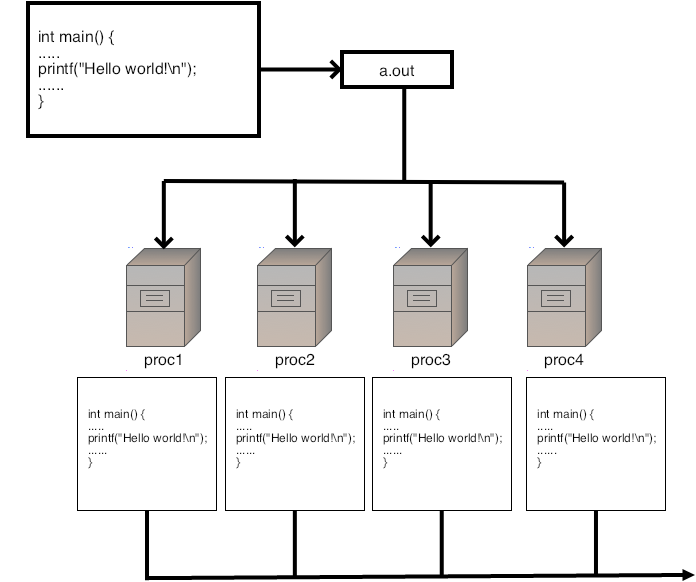
\includegraphics[scale=.5]{graphics/hello-parallel}
  \caption{Running a hello world program in parallel}
  \label{fig:rank-parallel}
\end{figure}
%
In other words, each process can find out `I~am process~5
out of a total of~20'.

%pyinput ex-rank.txt

\begin{exercise}
  \label{ex:hello3}
  Write a program where each process prints out a message
  reporting its number, and how many processes there are:
\begin{verbatim}
Hello from process 2 out of 5!
\end{verbatim}

  Write a second version of this program, where each process opens a
  unique file and writes to it. \emph{On some clusters this may not be
    advisable if you have large numbers of processors, since it can
    overload the file system.}
\end{exercise}

\begin{exercise}
  \label{ex:hello4}
  Write a program where only the process with number zero
  reports on how many processes there are in total.
\end{exercise}
